%!TeX root =  ../../thesis.tex

\section{Tester}
Tester je umístěn v plastovém boxu na vrchní části je umístěn displej a klávesnice na ovládání a na přední části jsou konektory pro testovaní kabelů.\\

Na obrázku \ref{fig:tester}  je pohled na výsledné testovací zařízení z vrchu, kdy je vidět celé ovládací rozhraní.
\\
Obrázek \ref{fig:testerIO} ukazuje konektory, kdy první tři zleva jsou výstupní a zbylé jsou vstupní, neboli ty testované.

\begin{figure}[H]
	\centering
	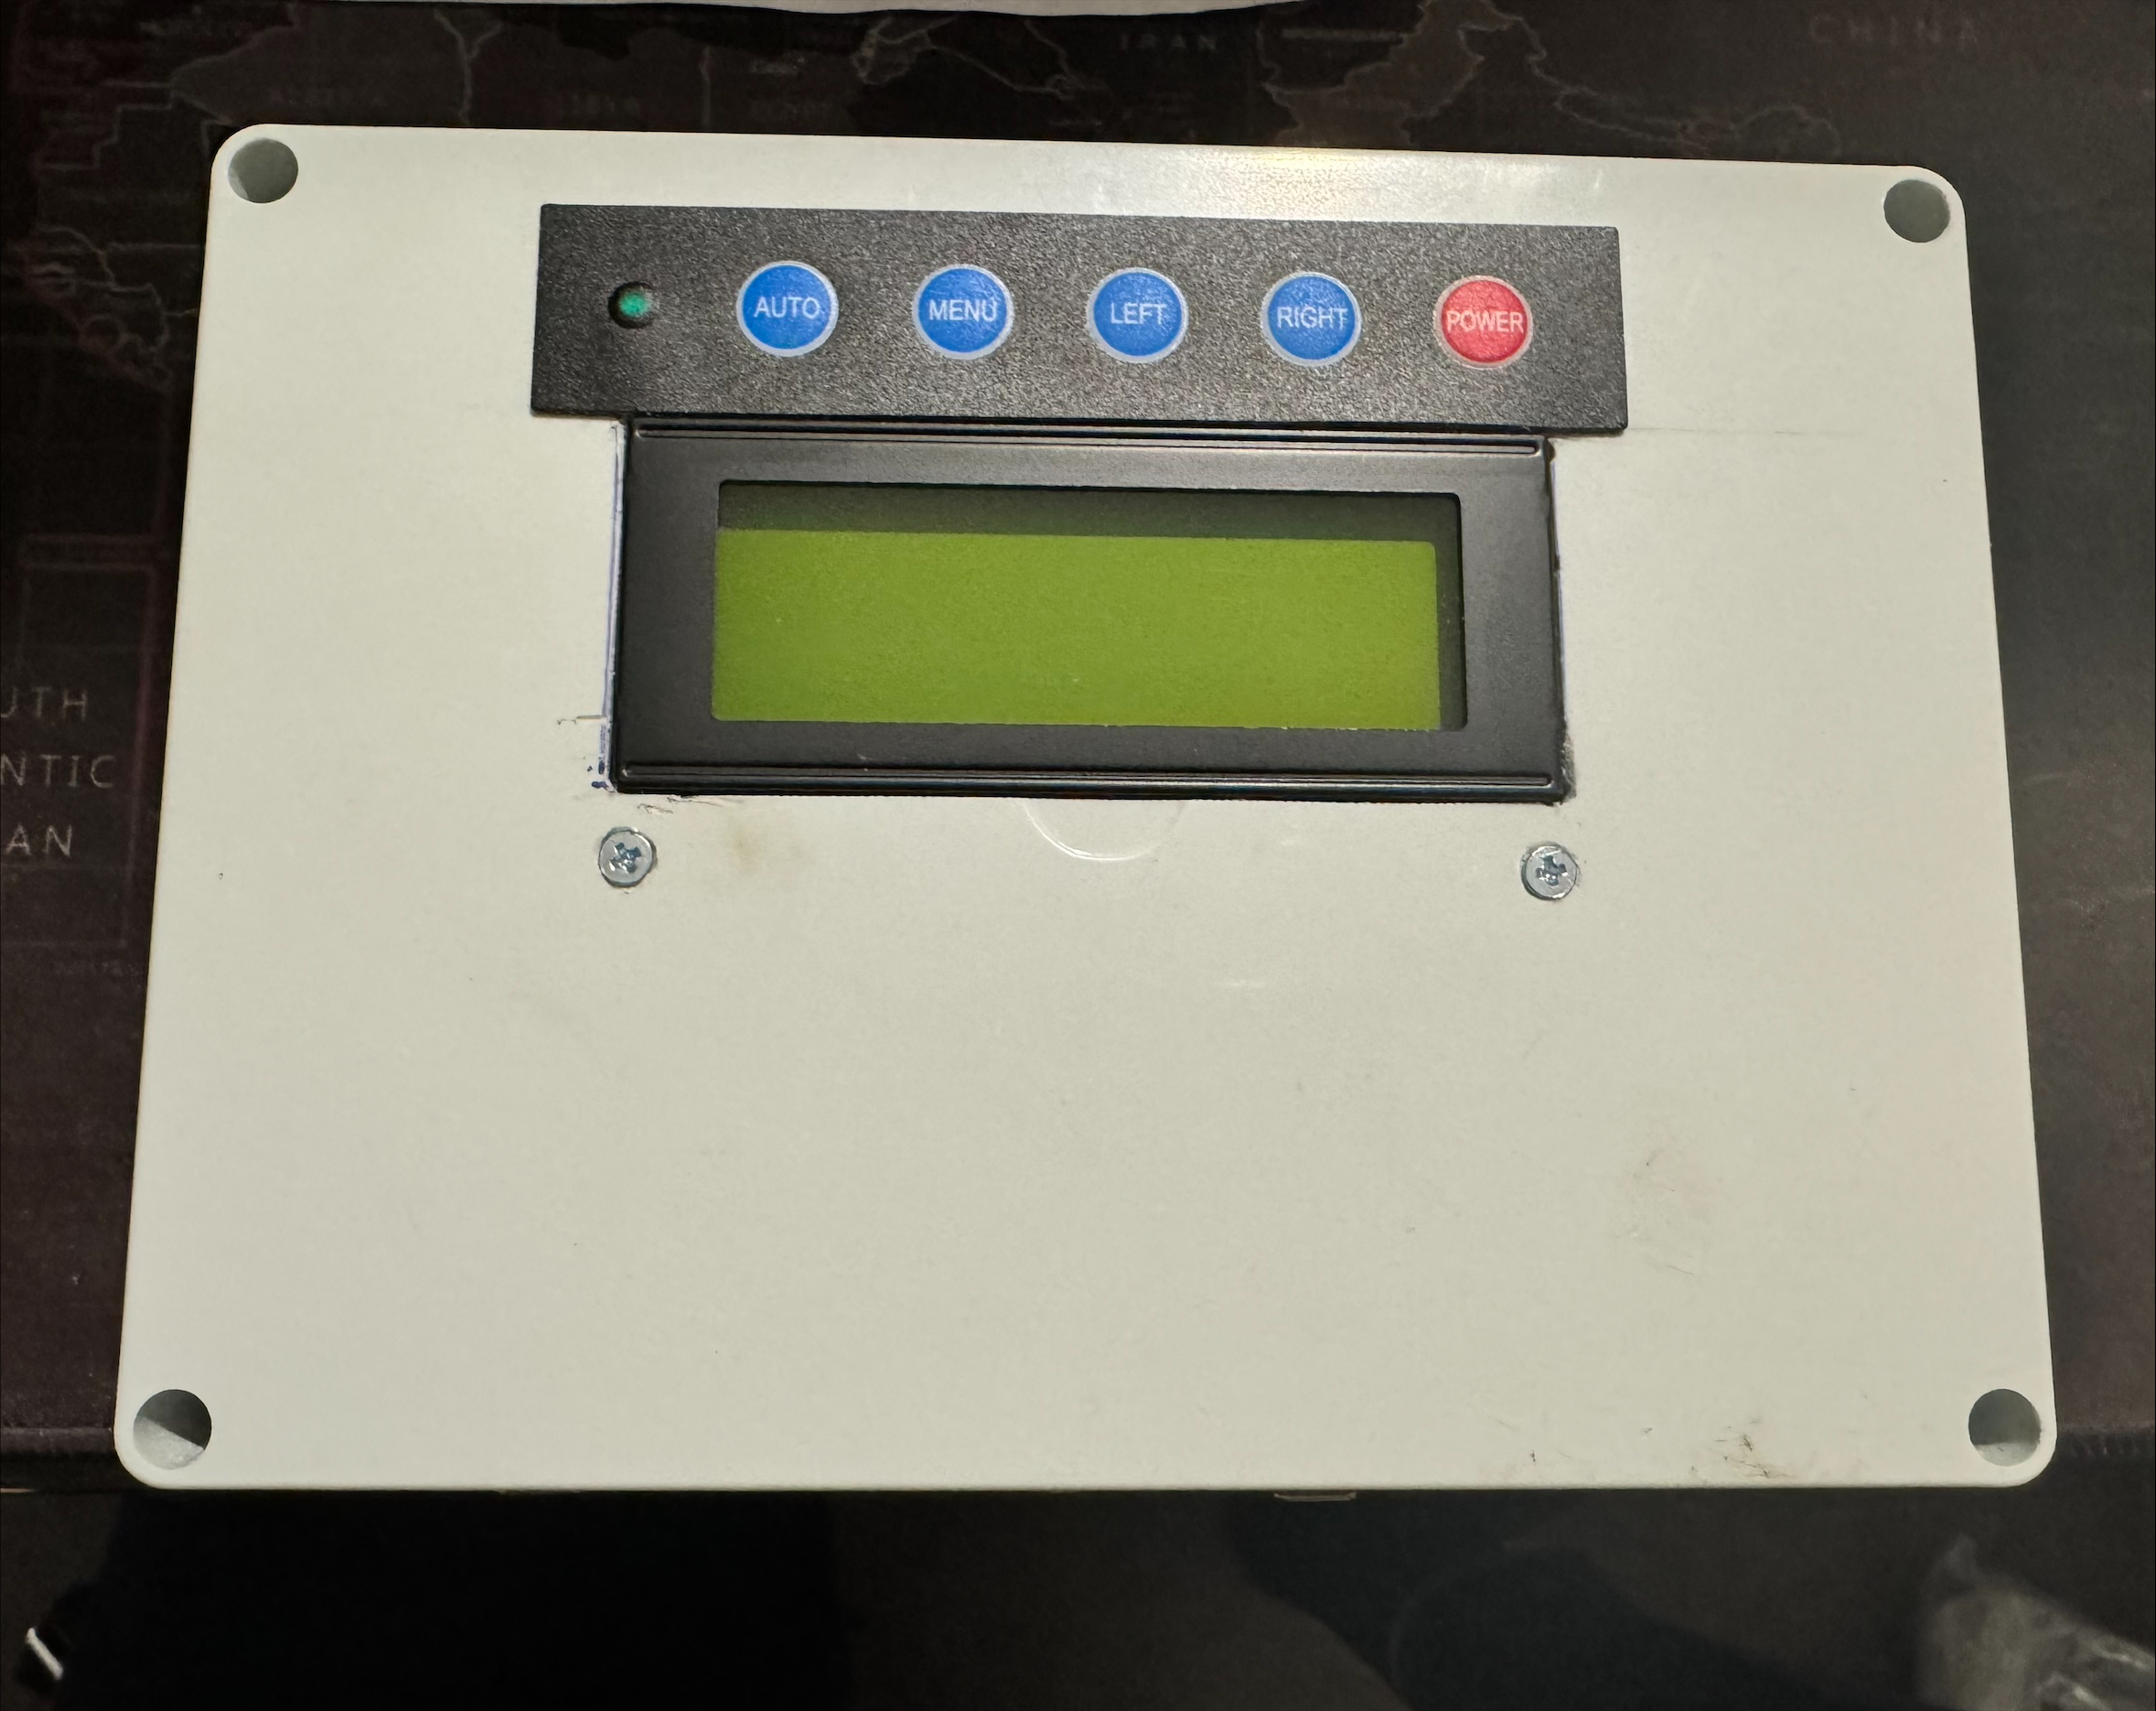
\includegraphics[width=0.9\textwidth]{pictures/tester-top.jpeg}
    	\caption{Výsledný tester na kabely}
   	\label{fig:tester}
\end{figure}

\begin{figure}[H]
	\centering
	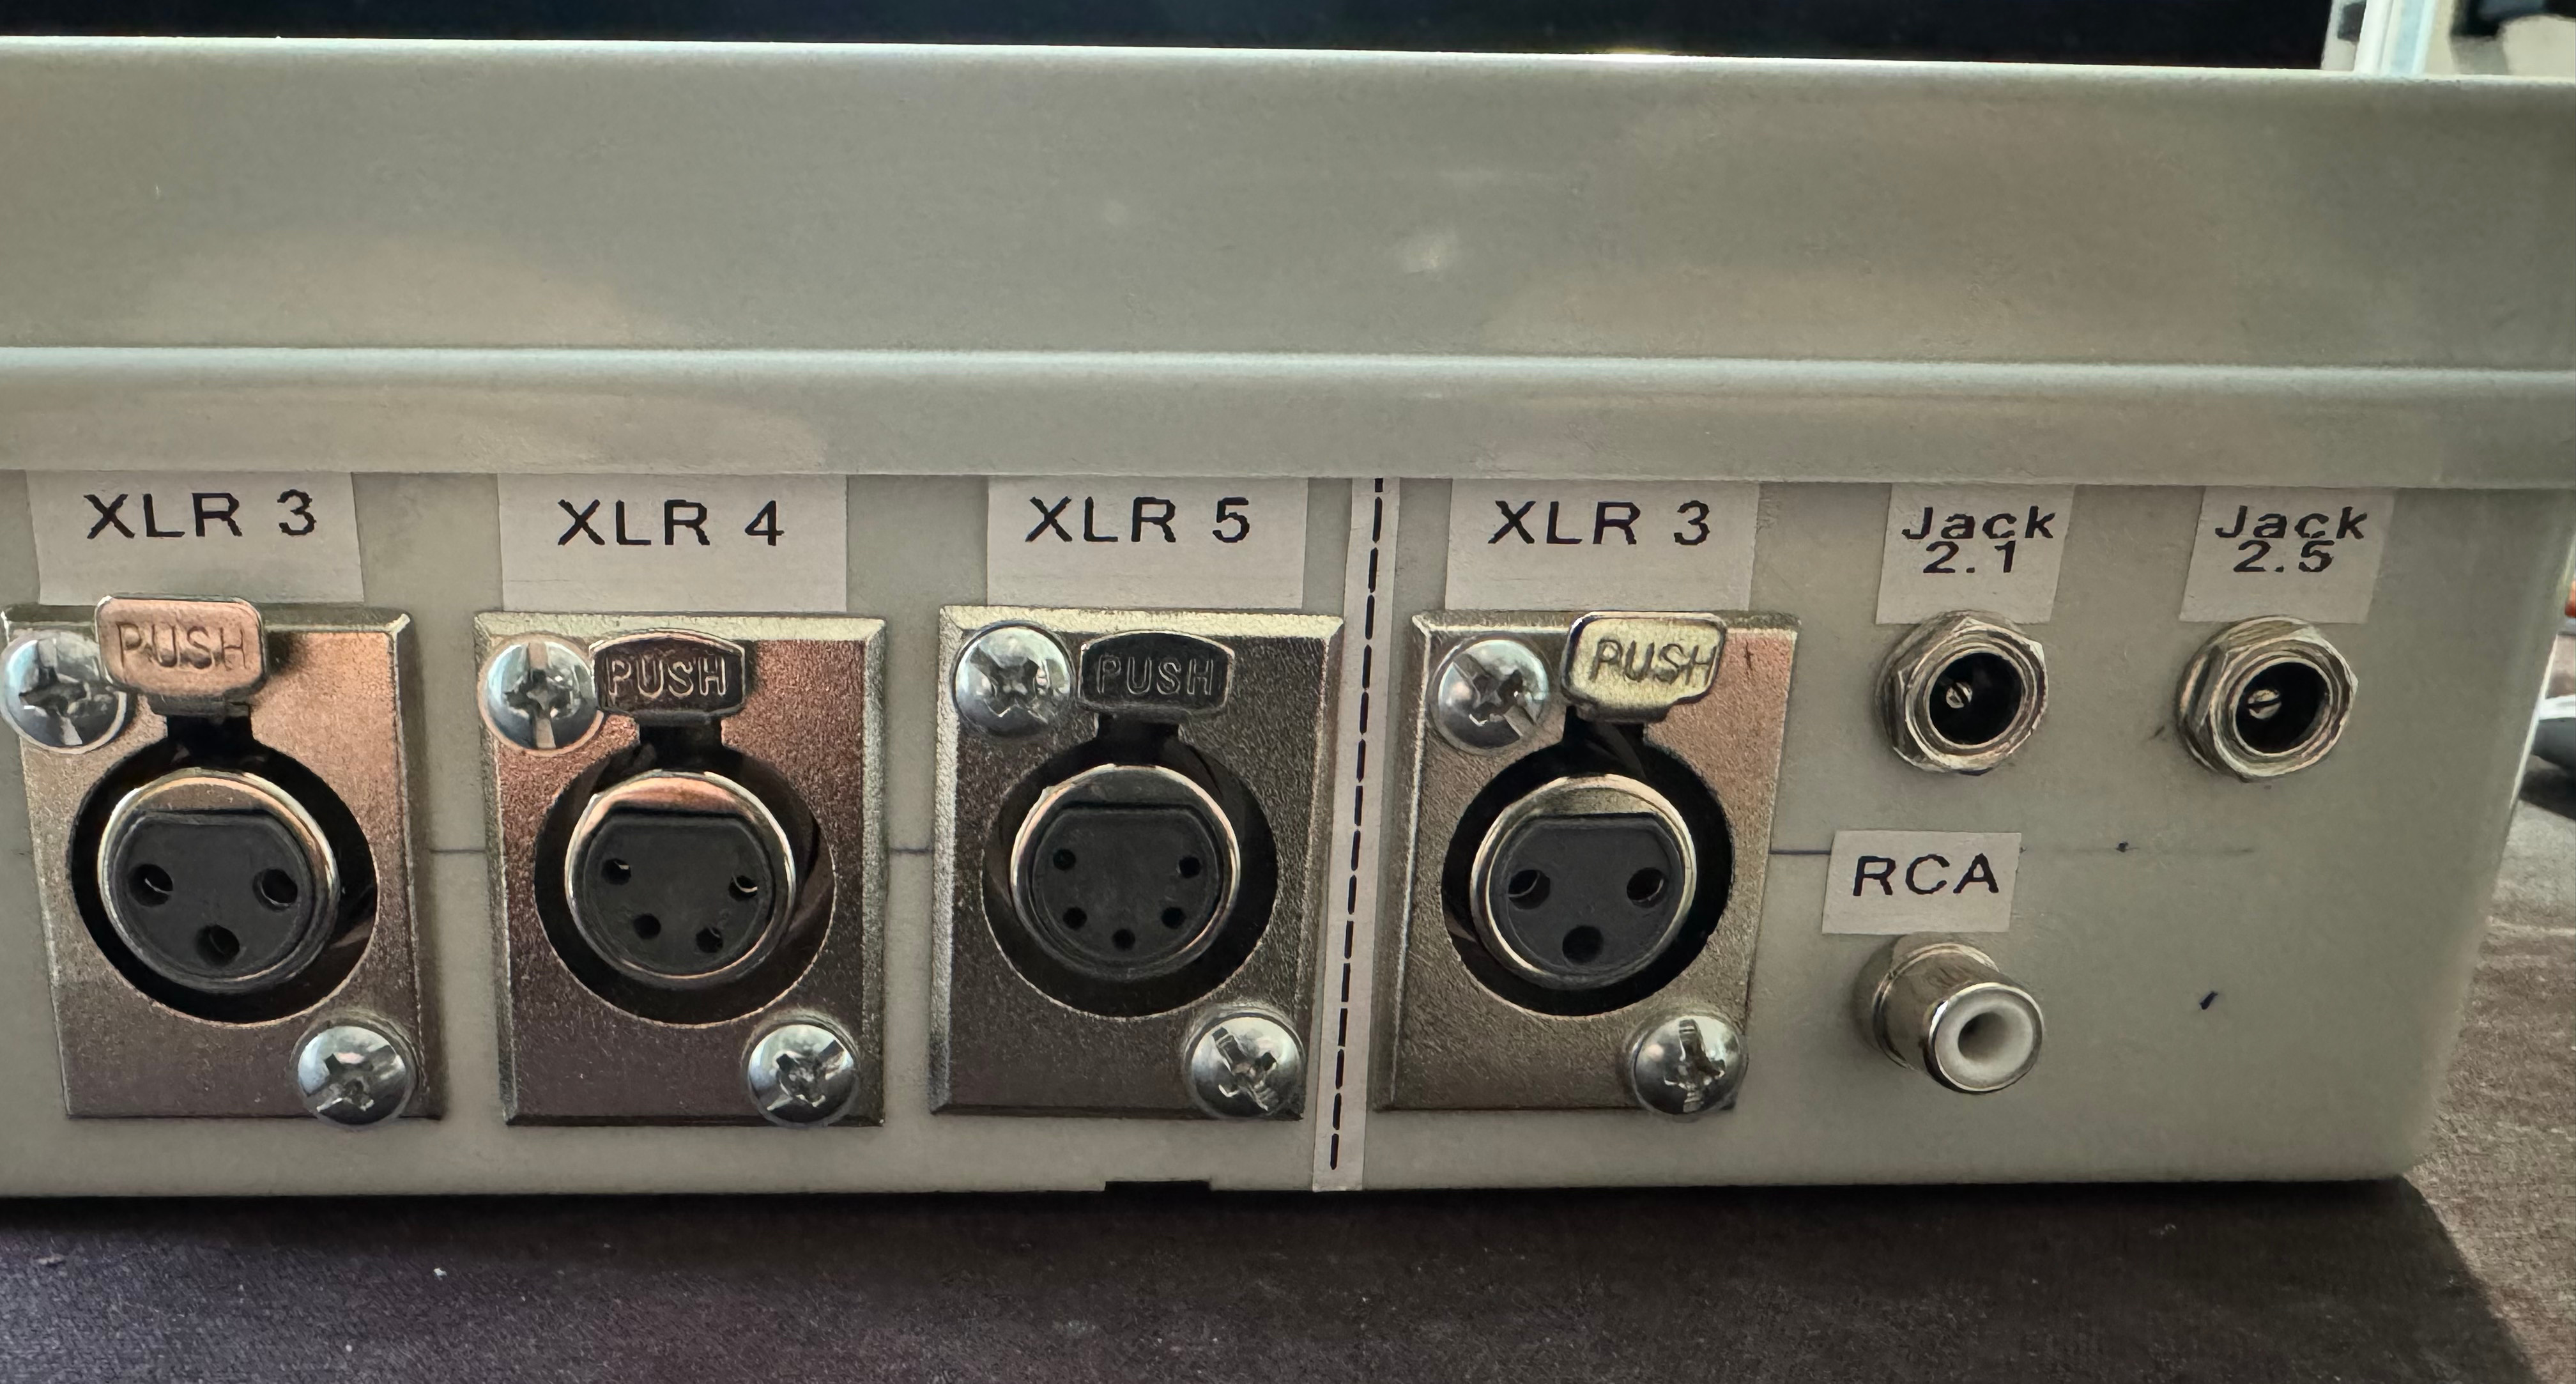
\includegraphics[width=0.9\textwidth]{pictures/tester-io.jpeg}
    	\caption{Výsledný tester na kabely}
   	\label{fig:testerIO}
\end{figure}

